
\section{Introduction}

This module will show how to use the mathematics of calculus, vectors, and
matrices to model and understand real physical systems. We will use Newtonian
dynamics to look at projectiles, elastic strings and springs, energy equations,
damped and forced oscillators, coupled oscillators, and Kepler's laws. We will
also study general nonlinear dynamical systems in two dimensions, which have
applications such as predator-prey systems in ecology. Often mathematical models
cannot be solved by purely analytical means. In this module we will also look at
how computational methods and analytical methods can complement each other to
help us understand and predict real world phenomena.


\section{Books}

\vspace{0.3cm}

{\small

\begin{tabular}{lp{5cm}p{5.5cm}}
\textbf{Collinson and Roper} * & \textbf{Particle Mechanics}          & Course book; strongly recommended; \\
%                               &      &         \\
\textbf{Dyke and Whitworth}    & \textbf{Guide to Mechanics}          & Nice, easy discussion    \\
%                               &      &         \\
\textbf{Smith and Smith}       & \textbf{Mechanics}                   & More advanced \\
%                               &      &         \\
\textbf{Lunn}                  & \textbf{A First Course in Mechanics} & Even more advanced \\
%                               &      &         \\
\textbf{Strogatz} *            & \textbf{Nonlinear Dynamics and Chaos} & Very clearly written with nice examples \\
%                               &      &         \\
%\textbf{Jordan and Smith}      & \textbf{Nonlinear Ordinary Differential Equations} & More advanced \\
%                               &      &         \\
\end{tabular}

}

\section*{Python Books}

\vspace{0.3cm}

{\small
\begin{tabular}{ll}
\textbf{Kong, Siauw and Bayen}   & \textbf{Python programming and numerical methods: A guide for engineers and scientists} \\
%                               &      &         \\
\textbf{Langtangen}             & \textbf{A primer on scientific programming with Python}  \\
\end{tabular}

}

\vspace{3mm}
\noindent
Most of these are available online - follow this links under the
Access your Reading List tile on ELE.

%\newpage



\section{Overview of Mathematical Modelling}


This module will introduce you to some of the kinds of mathematical models
that are used to understand and predict the behaviour of the real world,
along with some of the analytical and computational techniques used to
solve those mathematical models or understand their behaviour.

\begin{marginfigure}[1.4cm]
\begin{center}

\includegraphics[width=3.5cm]{IsaacNewton.png}
\end{center}
\caption{Isaac Newton lived from 1642 to 1727.}
\label{fig:IsaacNewton}
\end{marginfigure}


Some types of mathematical models are based on physical principles that
are so well established that they are considered to be `Laws of Nature';
Newton's Laws of Motion and his  Law of Universal Gravitation are examples
that we will look at (though they are now considered to be approximations
to deeper theories). 
Newtonian Dynamics is expressed in the
language of mathematics, and makes heavy use of calculus, vectors, and matrices.
Indeed, Newton's need to understand and apply his own theory helped to stimulate the
development of calculus (Fig.~\ref{fig:NewtDyn}).

\begin{figure}  %[!h]
  \hspace{-1cm}
  \vspace{3mm}
  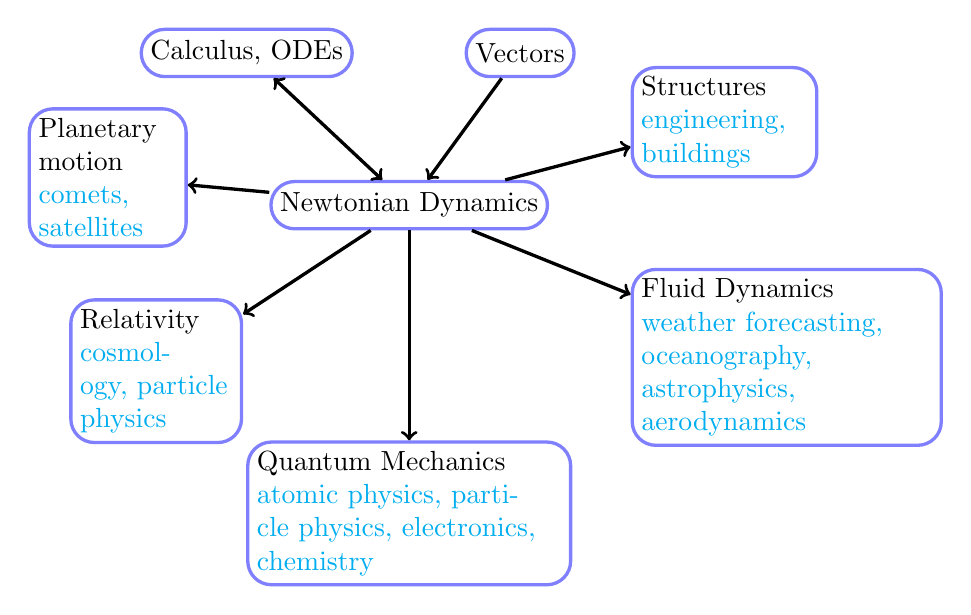
\begin{tikzpicture}[node distance=5mm,
      terminal/.style={
        % The shape:
        rectangle,minimum size=6mm,rounded corners=3mm,
        % The rest
        very thick,draw=blue!50}]
    \node(nd)[terminal]{Newtonian Dynamics};
    \node(calc)[terminal, above=55pt, left=20pt]{Calculus, ODEs};
    \node(vec)[terminal, above=55pt, right=20pt]{Vectors};
    \node(struc)[terminal, above=30pt, right=80pt, text width=60pt]{Structures \textcolor{cyan}{engineering, buildings}};
    \node(fd)[terminal, below=55pt, right=80pt, text width=105pt]{Fluid Dynamics \\ \textcolor{cyan}{weather forecasting, oceanography,\\ astrophysics,\\ aerodynamics}};
    \node(qm)[terminal, below=85pt, text width=110pt]{Quantum Mechanics \textcolor{cyan}{atomic physics, particle physics, electronics, chemistry}};
    \node(rel)[terminal, below=60pt, left=60pt, text width=55pt]{Relativity \textcolor{cyan}{cosmology, particle physics}};
    \node(plan)[terminal, above=10pt, left=80pt, text width=50pt]{Planetary motion \textcolor{cyan}{comets, satellites}};
    \path (nd) edge[very thick, <->] (calc);
    \path (nd) edge[very thick, <-] (vec);
    \path (nd) edge[very thick, ->] (struc);
    \path (nd) edge[very thick, ->] (fd);
    \path (nd) edge[very thick, ->] (qm);
    \path (nd) edge[very thick, ->] (rel);
    \path (nd) edge[very thick, ->] (plan);
  \end{tikzpicture}
  \caption{
    %Relation of Newtonian dynamics to some other topics.
    Newton's three laws of motion are the basis for Newtonian
    dynamics. In turn, Newtonian dynamics provides the basis for many
    areas of modern physics and engineering.  }
  \label{fig:NewtDyn}
\end{figure}

Other types of mathematical model are rather more
empirical, though they can still be extremely useful. Examples that we will
look at include Lotka-Volterra models for population dynamics, and the SIR
model for the spread of an epidemic.
\begin{marginfigure}[-25mm]

\includegraphics[width=4.5cm]{lotkavolterra.png}
\caption{\label{fig:lotka}
A model of competing populations.}
\end{marginfigure}

\begin{marginfigure}[5mm]

\includegraphics[width=4cm]{butterfly.png}
\caption{\label{fig:butterfly}
A solution trajectory for the Lorenz equations.}
\end{marginfigure}
The term {\bf Dynamical System} can refer to any system with time
dependence.  Examples include Newtonian dynamics, population dynamics,
the spread of infectious diseases, semi-conductor lasers,
biochemistry, and simplified models of more complex systems... See
figures \ref{fig:lotka} and \ref{fig:butterfly} for examples.

\vspace{20mm}

\eg{To make progress as applied mathematicians we must work with {\bf
    approximate models}. E.g., consider a car on a rollercoaster.
  What factors affect the motion?}

\begin{figure*}
\hspace{-1cm}

\includegraphics[width=12cm]{rollercoaster.png}
\caption{\label{fig:rollercoaster}
Schematic of a simple rollercoaster.
}
\end{figure*}

\noindent
Which factors are the most important? Which are completely negligible in practice?


\vspace{5mm}
In some cases (actually rather rare in the messy real world) we can
solve a mathematical model using analytical methods, for example based on
calculus, vectors, or matrices, and obtain a complete description of the
system's behaviour. Sometimes we cannot solve the mathematical model
exactly by analytical methods, but we may be able to make useful statements
about equilibria and their stability, or long term behaviour, or find approximate
solutions in special limiting cases. Often we will be able to obtain approximate solutions
using computational methods. We will look at many examples of how analytical
and computational methods complement each other in mathematical modelling.


Figure~\ref{fig:process} summarizes the modelling process. By making suitable approximations,
we construct a mathematical model of the system we wish to model. If we are lucky we may be able
to solve the equations analytically, or at least deduce qualitative properties of the
solution. Otherwise, we may be able to apply numerical methods to obtain an approximate
solution for the mathematical model. There is interesting mathematics behind designing,
analysing, and testing numerical models too.

\begin{figure}
  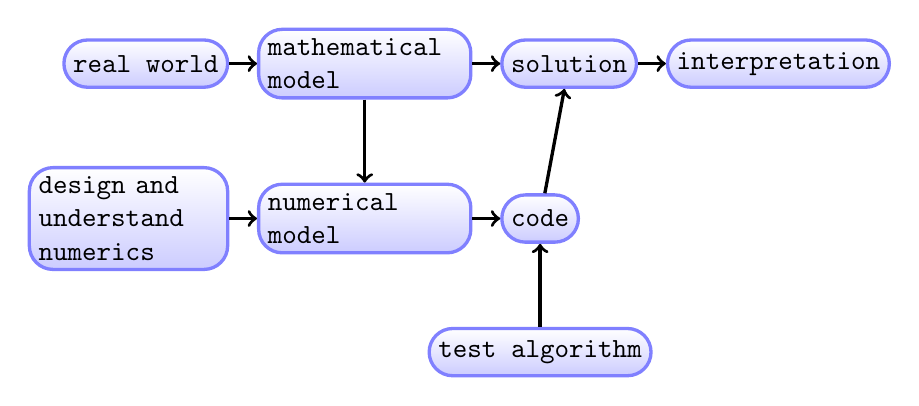
\begin{tikzpicture}[node distance=5mm,
      terminal/.style={
        % The shape:
        rectangle,minimum size=6mm,rounded corners=3mm,
        % The rest
        very thick,draw=blue!50,
        top color=white,bottom color=blue!20,
        font=\ttfamily}]
    \node(rw)[terminal]{real world};
    \node(mm)[terminal, right=10pt, at=(rw.east), text width=70pt]{mathematical model};
    \path (rw) edge[very thick, ->] (mm);
    \node(sol)[terminal, right=10pt, at=(mm.east)]{solution};
    \path (mm) edge[very thick, ->] (sol);
    \node(interp)[terminal, right=10pt, at=(sol.east)]{interpretation};
    \path (sol) edge[very thick, ->] (interp);
    \node(num)[terminal, below=30pt, at=(mm.south), text width=70pt]{numerical model};
    \path (mm) edge[very thick, ->] (num);
    \node(code)[terminal, right=10pt, at=(num.east)]{code};
    \path (num) edge[very thick, ->] (code);
    \path (code) edge[very thick, ->] (sol);
    \node(test)[terminal, below=30pt, at=(code.south)]{test algorithm};
    \path (test) edge[very thick, ->] (code);
    \node(design)[terminal, left=10pt, at=(num.west), text width=65pt]{design and understand numerics};
    \path (design) edge[very thick, ->] (num);

  \end{tikzpicture}
  \caption{\label{fig:process}
    Some steps in the modelling process.}
\end{figure}

%\noindent
%[{\bf Aside:}
\marginnote[-2cm]
{Think about what is meant by a {\bf model}. What is it that a mathematical model,
a computer model, a statistical model, and an airfix model have in common?}


This module assumes no prior knowledge of dynamics, mechanics, or physics.
Nor does it assume any prior knowledge of programming.
It does assume some prior knowledge of calculus, vectors, and complex numbers.


\section{Python: introduction}

To learn about computational methods in mathematical modelling we will
use the language \textbf{Python}. The key concepts behind coding in
Python are the same as those behind many other programming languages,
so once you are proficient in Python you should find it fairly
straightforward to pick up other languages.

In the first few weeks of this module we will spend some time learning
enough Python to be able to do something interesting.


\begin{enumerate}

\item
You can use Python on any PC across the University, in particular
during our computer practical laboratory sessions. You need to launch
Anaconda Navigator and we will use Jupyter Lab for interactive python
coding (using the iPython terminal) and also for writing python
scripts (\texttt{.py} files).
\item
If you have your own laptop or desktop you can install Anaconda following the instructions \href{https://www.anaconda.com/download}{here}.
\end{enumerate}


There are many excellent resources for learning Python. See, for
example, some of the books on the reading list and links under the
Python tile on ELE.


\section{Python: Arithmetic on the command line}

You can use Python in `interactive' mode by following these instructions:

\marginnote{
  Note the difference between the Powershell terminal and the iPython terminal. In the Powershell Terminal you can use commands to interact with the filesystem (we do not cover this in this module) or to run scripts (e.g. to run some Python code you have saved in a file; we shall see this later). The Powershell terminal does not know how to parse Python commands. In the iPython terminal we \textit{can} use Python commands. If you are typing Python commands into a terminal window and seeing \texttt{syntax error} messages, you may still be in the Powershell terminal, in which case, you need to type \texttt{ipython} and hit enter to open the iPython terminal.
  
  \vspace{10mm}

  Python commands will be indicated by \texttt{>>}. These characters are not part of the command and should not be typed in.
}

\begin{enumerate}
  \item First start Anaconda Navigator - you can find this by typing in the
    search box.
  \item \textbf{Wait patiently} for it to finish setting up (observe
    the progress bar at the bottom of the window) otherwise you may
    have some unpleasant errors!
  \item Scroll down to find `Jupyter Lab' and click the `Launch'
    button. Note, you do \textit{not} want `Jupyter Notebook'.
  \item When asked what type of file to open, choose `Terminal'. This
    will open a Powershell terminal (as we are using Windows machines)
    where you can interact with the filesystem using commands. We will
    only see a few basic command-line instructions, but for now...
  \item ...we will start an Interactive Python (iPython) session by typing
    \texttt{ipython} in the Terminal and hitting enter.
  \item Note that to exit iPython you press \texttt{ctrl-d} and hit
    \texttt{enter}.
\end{enumerate}

You can type instructions at the command line prompt to tell Python to
carry out basic arithmetic operations: addition (\verb!+!),
subtraction (\verb!-!), multiplication (\verb!*!), division
(\verb!/!), and exponentiation (\verb!**!).  Note that all
multiplications need to be written out explicitly: {\tt 2x} will give
an error, whereas {\tt 2*x} or {\tt x*2} is correct ({\tt x2} will be
seen as a new variable name; see below).

\eg{Compute the volume of a pyramid of height $150 \, \mathrm{m}$ and base area
$50000 \, \mathrm{m}^2$.}

\marginnote{
\texttt{>> 150*50000/3}
}

\eg{Compute the surface area of a cylinder of length $0.1 \,
  \mathrm{m}$ and radius $0.05 \, \mathrm{m}$.}

%\noindent
\marginnote{
\texttt{>> 2*pi*0.05*0.1 + 2*pi*0.05**2}
}

\vspace{5mm}
\noindent
Note that Python has a variable called \verb!pi!, which can be
imported from the \texttt{math} module (see next section) and takes
the value $3.14159265\ldots$.

We can use parentheses to group terms together, so for this last example we could have typed

%\noindent
\marginnote{
\texttt{>> 2*pi*0.05*(0.1 + 0.05)}
}
\noindent
Note that we refer to \emph{parentheses} as the round brackets  {\tt ()} on your keyboard. 
These are different from square brackets {\tt []} or curly brackets {\tt \{\}}. Computer languages are
fussy in this regard so make sure you use round brackets for mathematical expressions, and 
of course every opening bracket, {\tt (}, needs a matching closing bracket, {\tt )}. 

Just as in pencil-and-paper mathematics, exponentiation has a higher \textit{precedence}
than multiplication and division, which have a higher precedence than addition and subtraction.
For example,

%\noindent
\marginnote{
\texttt{>> 5*3**2}
}

\noindent
gives the result $45$, not $225$. If we really want to multiply $5$~by~$3$ before raising to
the power~$2$ then we should include parentheses, which take precedence over everything else:

%\noindent
\marginnote{
\texttt{>> (5*3)**2}
}

\noindent
Addition and subtraction have equal precedence. Multiplication and division have equal precedence.
This means that expressions like 

%\noindent
\marginnote{
\texttt{>> 20/10*2}
}

\noindent
are potentially ambiguous if we forget whether Python works left-to-right or right-to-left.
In such cases it is better to rearrange the formula or use parentheses to resolve the ambiguity:

%\noindent
\marginnote{
\texttt{>> 20/(10*2)} \ \ \ \ or \ \ \ \ \texttt{>> (20/10)*2}
}
\noindent
(In fact Python interprets {\tt 20/10*2} as $\frac{20}{10} \times 2 = 4$, which shows the 
care that is needed here.)

Very large or very small numbers can be represented using `\texttt{e}' notation.

\eg{How far does light (speed $3 \times 10^8 \, \mathrm{ms}^{-1}$)
  travel in one year ($3.15 \times 10^7 \, \mathrm{s}$)?}

\marginnote{
\texttt{>> 3e8*3.15e7}
}

\eg{Roughly how many protons (mass $1.67 \times 10^{-27} \, \mathrm{kg}$)
make up the mass of the sun (mass $2 \times 10^{30} \, \mathrm{kg}$)?}

\marginnote{
\texttt{>> 2e30/1.67e-27}
}

\section{Python: The \texttt{math} and \texttt{cmath} modules; variables}
\label{sec:built-in}

Python keeps things tidy by collecting objects such as functions
together in modules. For example, the \texttt{math} module contains
the definitions of a lot of mathematical functions and useful
constants such as $\pi$. To access these definitions, we need to import
them from the module: \\

\texttt{>> from math import pi} \\

The \href{https://docs.python.org/3/library/math.html}{\texttt{math}}
and
\href{https://docs.python.org/3/library/cmath.html}{\texttt{cmath}}
modules contain functions to compute many standard mathematical
functions. The \texttt{math} functions are only defined for real input
and output, whereas the \texttt{cmath} functions will accept real and
complex input (where appropriate) and, importantly, will
\textit{always} return a complex number. Table~\ref{tab:builtin} below
lists some of those most commonly used. Note that the input argument
to the function is specified in parentheses. Note also that the input
arguments to trig functions (and the outputs of their inverses) are in
radians.  There is no function called {\tt ln}; for natural logarithm
you must use {\tt log} and for log base 10 you use {\tt log10}; this
is common to scientific computer languages.


\hspace{-10mm}
\begin{table}
\caption{\label{tab:builtin} Some commonly used mathematical Python functions.}
\begin{tabular}{|p{20mm} p{40mm} | p{20mm} p{40mm}|}
% Leave two blank rows to fit in the caption!
\multicolumn{4}{c}{}\\
\multicolumn{4}{c}{}\\
\toprule
\texttt{sin(x)}   & Standard trig functions   & \texttt{sqrt(x)}    & Square root  \\
\texttt{cos(x)}   &                           & \texttt{exp(x)}     & $\ee^x$      \\
\texttt{tan(x)}   &                           & \texttt{log(x)}     & Natural logarithm \\
\texttt{asin(x)}  & Their inverses            & \texttt{log10(x)}   & Base~10 logarithm \\
\texttt{acos(x)}  &                           & \texttt{abs(x)}     & $|x|$         \\
\texttt{atan(x)}  &                           & \texttt{factorial(x)} & $x!$ \\
\texttt{sinh(x)}  & Hyperbolic trig functions & \texttt{round(x)}   & Round to nearest integer \\
\texttt{cosh(x)}  &                           & \texttt{floor(x)}   & Round down     \\
\texttt{tanh(x)}  &                           & \texttt{ceil(x)}    & Round up       \\
\texttt{asinh(x)} & Their inverses            &  & \\
\texttt{acosh(x)} &                           &  & \\
\texttt{atanh(x)} &                           &  & \\
\bottomrule
\end{tabular}
\end{table}


\eg{Find the roots of the quadratic equation $x^2 + 7x + 2 = 0$.}

\marginnote{
\texttt{>> (-7 + sqrt(7*7 - 4*2))/2}
}
\marginnote{
\texttt{>> (-7 - sqrt(7*7 - 4*2))/2}
}

\eg{Two adjacent sides of a triangle have lengths $4 \, \mathrm{m}$
  and $5 \, \mathrm{m}$ and the angle between them is $2$~radians;
  find the length of the third side.}

\marginnote{
\texttt{>> sqrt(4**2 + 5**2 - 2*4*5*cos(2))}
}

We can store numbers, including the results of calculations, in named locations in the
computer memory, called \textbf{variables}, to use them later. This is very useful when
the calculation involves several, or many, steps.
The example we have just seen could be solved thus:

\marginnote{
\texttt{>> a = 4}
}

\marginnote{
\texttt{>> b = 5}
}

\marginnote{
\texttt{>> C = 2}
}

\marginnote{
\texttt{>> sqrt(a**2 + b**2 - 2*a*b*cos(C))}
}

\noindent
Note that this is clearer and easier to read and check mathematically, than
the earlier version with the numbers inserted in place of {\tt a}, {\tt b}, {\tt C}. It is also
easier to test and reuse with different values, when we introduce \textbf{scripts} 
below. Also note the judicious use of spaces to 
help the eye to see the structure of the equation: you should experiment with 
putting in space to make lines more readable for you --- there is no right or wrong way to do this.

\vspace{6mm}
\noindent
Variable names must start with a letter, followed by any number of
letters, digits, or underscore characters. It is a good idea
\textit{not} to use variable names that are already the names of
built-in Python functions as this can lead to unexpected behaviour
that is difficult to debug.

\vspace{5mm}
\noindent
Note that variable names are case sensitive: \texttt{Temp} is a different variable from
\texttt{temp}, etc.

\eg{In a simple mathematical model for the spread of an epidemic,
  called the SIR model, $S(t)$ is the number of susceptible people,
  i.e.\ those who have not yet had the disease, $I(t)$ is the number
  of infected people, and $R(t)$ is the number removed from the system
  (recovered or deceased). Their respective initial values are $S_0$,
  $I_0$, and $R_0 = 0$.  The governing equations are}
%begin{eqnarray}
%\frac{d S}{d t} & = & -r I S ; \nonumber \\
%\frac{d I}{d t} & = & r I S - a I ; \nonumber \\
%\frac{d R}{d t} & = & a I . \nonumber
%\end{eqnarray}
\begin{equation}
\frac{d S}{d t} = -r I S ; \qquad \frac{d I}{d t} = r I S - a I ; \qquad \frac{d R}{d t} = a I .
\end{equation}
Here $r$ and $a$ are constants; $r$ is the reproduction rate and $1/a$ is the average time a person
is infected.
These equations cannot be solved exactly in general, but it can be shown
(see section~\ref{sec:SIR}) that the peak in the number of infected people is
given by
\begin{equation}
\label{eq:Imax}
I_\mathrm{max} =
\left\{
\begin{array}{ll}
I_0 + S_0 - \frac{1}{q} \left\{\ln (q S_0) + 1 \right\} & \mathrm{if\ }qS_0 > 1 \\
I_0                                                     & \mathrm{otherwise}
\end{array}
\right.
\end{equation}
where $q = r/a$, 
while the number of people removed from the system when the epidemic eventually dies out
is
\begin{equation}
\label{eq:Rend}
R_\mathrm{end} = S_0 + I_0 - S_\mathrm{end}
\end{equation}
where $S_\mathrm{end} $ satisfies the implicit equation
\begin{equation}
\label{eq:Send}
S_\mathrm{end} - \frac{1}{q} \ln S_\mathrm{end} = I_0 + S_0 -\frac{1}{q} \ln S_0 .
\end{equation}
For the parameters $I_0 = 1000$, $S0 = 6 \times 10^7$, $r = 3 \times 10^{-9} \, \mathrm{day}^{-1}$,
$a = 1/(14 \, \mathrm{day})$, determine the maximum number of infected people. 
In this case you need to check that $qS_0>1$ so as to apply the correct formula in
(\ref{eq:Imax}):

\marginnote{
\texttt{>> I0 = 1000}
}

\marginnote{
\texttt{>> S0 = 6e7}
}

\marginnote{
\texttt{>> q = 3e-9*14}
}

\marginnote{
\texttt{>> q*S0}
}

\marginnote{
\texttt{>> Imax = I0+S0 - (1+log(q*S0))/q}
}

\vspace{18mm}
Apart from integers and real numbers, which we have seen already, Python can work with
complex numbers (always use {\tt 1j} and never {\tt j} for the square root of $-1$)...

\marginnote{
\texttt{>> q = (1 + 3j)**2}
}
\marginnote{
\texttt{>> z = exp(1j*pi)}
}

\vspace{10mm}
\noindent
logicals ...

\marginnote{
\texttt{>> sun = True}
}
\marginnote{
\texttt{>> weekend = True}
}
\marginnote{
\texttt{>> bbq = sun and weekend}
}

\vspace{10mm}
\noindent
and character strings.

\marginnote{
\texttt{>> subject = 'Modelling'}
}

\vspace{10mm}
All variables are cleared at the end of an iPython session To save
your session commands for future reference, type \texttt{\%save
  filename}. This will save the commands up to that point in a file
called \texttt{filename.py} (you can choose any filename but don't
include spaces or special characters). You will find it helpful to
create a directory in OneDrive called MTH1003 for storing files
related to this module.

\section{Python: assignment, sequences of commands}

There is a crucial conceptual difference between the use of `=' in pencil-and-paper
mathematics and the use of `=' in a programming language such as Python. In
pencil-and-paper mathematics, $y = x^2 +4x + 5$ is an \textit{equation}, a statement
that the left hand side is equal to the right hand side, at least for the duration of
the calculation at hand. In Python, on the other hand, \texttt{y = x**2 + 4*x + 5}
is an \textit{instruction}; it means evaluate the expression on the right hand side
and \textit{assign} the result to the variable whose name appears on the left hand side.
Now it will be true that the value of \texttt{y} is equal to the value of 
\texttt{x**2 + 4*x + 5} immediately after the instruction is executed, but it will cease
to be true as soon as a subsequent instruction assigns a different value to~\texttt{y}
(or~\texttt{x}).

On a closely related point, we must remember that Python executes the commands we
give one at a time, in the order we give them. The values of the variables change
as each command is executed. These ideas become particularly important
when we come to write scripts and functions.
Thus, while in pencil-and-paper mathematics it would be nonsensical to write $p = 6$, $p = 7$,
$p = p + 1$, the following is a perfectly valid and meaningful sequence of Python commands:

\marginnote{
\texttt{>> p = 6}
}

\marginnote{
\texttt{>> p = 7}
}


\marginnote{
\texttt{>> p = p + 1}
}

\ex{ What are the values of \texttt{a} and \texttt{b} after each of
  the following commands?  Try to work it out yourself before checking
  using Python.}

\marginnote{
\texttt{>> a = 3}
}

\marginnote{
\texttt{>> b = 4}
}

\marginnote{
\texttt{>> a = a + b}
}

\marginnote{
\texttt{>> b = a - b}
}

\marginnote{
\texttt{>> a = a - b}
}

\vspace{10mm}


\section{Python: Precision}

Computers have finite memory, and this means they cannot store real numbers
such as $\pi$ or $\sqrt{2}$ exactly; such numbers can only be stored to
some finite \textit{precision}. By default Python stores real numbers to a
precision of about 15~decimal digits. 

\noindent
This is more than enough for most practical
purposes. However, there are certain calculations in which the effects of
tiny precision errors (also called \textit{roundoff errors}) are greatly
amplified, and it is as well to be aware of these.
Examples of such sensitive calculations include accumulating the sum of
many terms, taking small differences of relatively large numbers,
finding roots of polynomials, and certain eigenvalue computations.
\marginnote{
E.g.\ type

\texttt{>> 0.21 - 0.5 + 0.29}
}
See also Appendix~C.

\ex{Use Python with the usual roots of a quadratic formula to solve
  $x^2 - (10^p + 10^{-p}) x + 1 = 0$ for different~$p$. First find the
  exact roots by factorising the expression. How big does $p$ have to
  be before the standard quadratic formula calculation for these roots
  goes wrong? What is the issue and how could it be cured?}



\section{Linear interpolation}
\label{sec:linear_interp}

Suppose we are given some tabulated data, for example temperatures $T_i$ at certain heights
$z_i$ in the atmosphere, and we wish to estimate the temperature at an intermediate height
that is not tabulated. In effect we need to construct a \textit{mathematical model}
for the dependence of temperature on height between the tabulated values.

One class of mathematical model is \textit{interpolation}; it involves fitting a 
curve through the given data points. The simplest type of interpolation is
\textit{linear interpolation}, which fits a straight line between each neighbouring
pair of data points.
\begin{marginfigure}[-8mm]

\includegraphics[width=5cm]{USSA.png}
\caption{\label{fig:USA}
Data points defining the US Standard Atmosphere temperature profile
(black circles), and the temperature at $40 \, \mathrm{km}$ obtained
by linear interpolation (red filled circle).
}
\end{marginfigure}

Given two neighbouring data points $(x_1 , y_1)$, $(x_{2} , y_{2})$,
the equation of the straight line passing through these points is
\begin{equation}
y = \frac{(x - x_1) y_{2} + (x_{2} - x) y_1}{x_{2} - x_1}
\end{equation}
[exercise: check this].
Thus, an estimate $\hat{y}$ for the value of $y$ at $x = \hat{x}$ is given by
\begin{equation}
\label{eq:linear_interp}
\hat{y} = \frac{(\hat{x} - x_1) y_{2} + (x_{2} - \hat{x}) y_1}{x_{2} - x_1} .
\end{equation}

The closer our given data points are to each other, the more accurate
we might expect our interpolated value to be. Let's investigate this idea
empirically on a case for which we know the answer. We will try to estimate
the value of $\sin(1)$ by linearly interpolating between
$y_{1} = \sin(1 - h/3)$ and $y_{2} = \sin(1 + 2h/3)$ for different values
of $h$. Putting $x_1 = 1 - h/3$ and $x_{2} = 1 + 2h/3$ into \eqref{eq:linear_interp}
gives
\begin{displaymath}
\hat{y}
%= \frac{(h/3)\sin(1 + 2h/3) + (2h/3)\sin(1 - h/3)}{h}
= \frac{1}{3}\sin(1 + 2h/3) + \frac{2}{3}\sin(1 - h/3) .
\end{displaymath}
For any value of $h$, the error in our estimate is $\varepsilon = |\hat{y} - \sin(1)|$.
We can use Python to see how the error depends on $h$.

\noindent
\texttt{>> h = 1}

\noindent
\texttt{>> yerr = abs( sin(1 + 2*h/3)/3 + sin(1 - h/3)*2/3 - sin(1) )}

\noindent
\texttt{>> h = h/2}

\noindent
\texttt{>> yerr = abs( sin(1 + 2*h/3)/3 + sin(1 - h/3)*2/3 - sin(1) )}
\marginnote{
Tip: use the up-arrow key to bring up commands entered previously
to save typing them again. You can also edit them before 
pressing return, so 
saving time and effort for repeated calculations.
}

\noindent
etc.

There is a way to rewrite the linear interpolation formula above, which is trivial yet very informative!
We rearrange the terms so it takes the form:
%
\begin{equation}
y = %y_1  \, \frac{x - x_{2}}{x_1-x_{2}}  + y_2 \, \frac{x - x_1}{x_{2} - x_1} = 
y_1 \, L_1(x) + y_2 \, L_2(x), 
\label{eq:lag1}
\end{equation}
%
with 
%
\begin{equation}
L_1(x) = \frac{x - x_{2}}{x_1-x_{2}} \,  , \quad L_2(x) = \frac{x - x_1}{x_{2} - x_1}\,  .
\label{eq:lag2}
\end{equation}
%
Now if we look at $L_1(x)$, it has the property that $L_1(x_1)=1$ and $L_1(x_2)=0$: it switches on at $x_1$ and off at $x_2$.  Similarly 
$L_2(x_2)=1$ and $L_2(x_1)=0$ and so $L_2$ switches on at $x_2$ and off at $x_1$. 

Thus one can see how the formula for $y(x)$ works to give a straight line that passes through $(x_1,y_1)$ and $(x_2,y_2)$, with the appropriate terms switching on and off when we put in $x=x_1$ and $x=x_2$ (check this out!). This gives a hint about how to generalise from linear interpolation between two points, for example to putting a cubic curve through four points; we will meet this later and it is known as \emph{cubic interpolation}. The $L_1$ and $L_2$ polynomials (here linear functions) are called \emph{Lagrange polynomials}, and we'll meet the more general form shortly. 

\section{Numerical analysis and Taylor--Maclaurin series}
\label{sec:Taylor_series}


\subsection{What is numerical analysis?}

We have met the numerical process of \emph{linear interpolation} for estimating values of a function given 
some dataset, and we will meet several other numerical methods during this module. Although we can, with
some work, write down a variety of methods of giving convincing answers to numerical problems, one key aspect
is to understand what \emph{errors} are made --- since none of these methods will generally give exact answers. Indeed
if we have two numerical methods for solving the same problem, we need to understand the size of the errors to know
which method is superior. This consideration then feeds into how we design accurate and robust methods.

The analysis of numerical methods, their errors and other properties, forms the subject of \emph{numerical analysis}, 
which is an important and vigorous topic in mathematics and computation. Huge investments go into numerical methods used 
for simulating weather, climate, satellites, galaxies, black holes, ..., and the design of aircraft, engines, wind farms .... all sorts of applications. 
A mathematical understanding of these methods is vital for society, particularly as computer architectures and capabilities change. 

\subsection{Taylor--Maclaurin series} 

We will only touch on the area of numerical analysis in this module, but hope to give you the basic ideas and tools that 
will be developed in the second year modelling module and beyond. For studying errors there is one key idea that we 
need to discuss, namely that of \emph{Taylor--Maclaurin series} and the related \emph{Taylor's theorem}. These are topics you will meet
in other modules, so you will revisit these ideas, but we will introduce them carefully here. 

First suppose we have a function $f(x)$ with derivative $f'(x)$ (we are taking $f$ to be differentiable). Suppose
we have a point $x=a$ and we wish to approximate $f(a+h)$ for nearby points $x = a+h$ (we are thinking of $h$ being small). 
Then graphically, thinking of the tangent line through the curve at $x$, we can approximate 
%
\begin{equation}
f(a+h)  \simeq f(a) + h f'(a).
\notag
\end{equation}
%
This gives a good approximation as long as $h$ is small, with some error which we'll discuss shortly. For example, consider
%
\begin{equation}
f(x) = \frac{1}{1+x}\, , \quad f'(x) = - \frac{1}{(1+x)^2} \, . 
\notag
\end{equation}
%
and the point $ x = a = 1$. We then have  $f(a) = f(1) = 1/2$, $f'(a) = f'(1) = - 1/4$, and so our approximation is 
 %
\begin{equation}
f(1+h)  \simeq  1/2  - h / 4 . 
\nonumber
\end{equation}
%
This is just a linear function of $h$, the line tangent to the curve at $x=a=1$. Two questions then arise --- what is the error 
in this approximation, and how can we do better? 

To do better we employ the generalisation of this, which uses more information on the rate of change of $f$ and $f'$ at $x$, and is:
%
\begin{equation}
f(a+h)  \simeq f(a) + h f'(a) + \frac{1}{2!} \, h^2 f''(a) .
\notag
\end{equation}
%
In our example $f''(x) = {2}/{(1+x)^3}$ and $f''(a) = f''(1) = 2/8 = 1/4$, giving
 %
\begin{equation}
f(1+h)  \simeq  1/2  - h / 4  + h^2/8 .
\notag
\end{equation}
%
This is the quadratic in $h$ that fits the curve $y=f(x)$ at $x=a=1$ in the best way.

What are the errors in these approximations? We define an error $\varepsilon$ in any approximation as
%
\begin{equation}
\varepsilon = \Big| \text{(approximate answer)} - \text{(exact answer)}   \Big|
\notag
\end{equation}
%
and so given the modulus signs, $\varepsilon$ is always positive or zero. %
\marginnote{Or, $\varepsilon$ is said to be \emph{non-negative}.} %
So for our linear approximation 
%
\begin{equation}
\varepsilon = \Big| \, 1/2  - h / 4    -  \frac{1}{2+h} \,\Big|.
\notag
\end{equation}
%
This depends on $h$, but say at $h=1$ we have $f(1+h) = 1/3$ and the approximation gives $1/4$ so $\varepsilon = 1/12$. The quadratic 
approximation gives an answer of $3/8$ and so the error is $\varepsilon = 1/24$. 



If we want to gain better and better approximations by including more terms we gain a \emph{Taylor--Maclaurin series}
%
%
%
\begin{eqnarray}
f(a+h) & = & f(a) + h f'(a)
   + \frac{h^2}{2!}f''(a) + \frac{h^3}{3!}f'''(a) + ... + \frac{h^{n}}{n!} f^{(n)}(a) + \cdots \nonumber   \\ 
 & = & \sum_{k=0}^{\infty}\,\, \frac{h^{k}}{k!}\, f^{(k)}(a) . \notag
   \label{eq:taylor_series0}
\end{eqnarray}
where the superscript $(k)$ means the $k^\mathrm{th}$ derivative.
%
\marginnote{Strictly this is a Maclaurin series if $a=0$ otherwise a Taylor series --- the 
difference is not essential (think of translating the function along the $x$-axis); we'll often refer to this as a Taylor series in either case.}%
%
For our example this results in:
 %
\begin{equation}
f(1+h)  =  1/2  - h / 4  + h^2/8  - h^{3}/16 + h^4/32 + \cdots , 
\notag
\end{equation}
%
%
\marginnote{In fact this series converges provided $|h| < 2$ and diverges otherwise. For general functions $f(x)$ the issue
of convergence of a Taylor series has important links to the behaviour of the corresponding function $f(z)$ of a 
complex variable $z$ and where the singularities of $f$ lie in the complex plane, as discussed in second year modules.}%
%
which is simply a binomial expansion. We have put an `equals sign' here, but that opens up the key question of when such series 
do --- in the limit of summing infinitely many terms --- give back our original function $f$. We will not
address this question here (see other, pure modules) but assume that such series work for reasonably
small values of $h$. 

\ex{Obtain the linear and quadratic approximations for the function
  $f(x) = \sin x$ \emph{about the point} $a = \pi/6$.}

\ex{Given that $f(x) = \cosh x = \tfrac{1}{2} (\ee^x + \ee^{-x})$ and
  $g(x) = \sinh x = \tfrac{1}{2} (\ee^x - \ee^{-x})$, show that $f'(x)
  = g(x)$ and $g'(x) = f(x)$.  Obtain the infinite Taylor--Maclaurin
  series for $f(x)$ about $a=0$. Compare this series with the
  well-known series for the cosine function, namely $\cos x = 1 -
  \tfrac{1}{2!} x^2 + \tfrac{1}{4!} x^4 - \cdots$.}

\subsection{Taylor's theorem}

We will find the following theorem useful, namely \emph{Taylor's theorem}, which tells us what we get if
we truncate the series and just sum the terms from $k=0$ to $k=n$. It turns out that the error we make is 
approximately a constant times $h^{n+1}$ \emph{provided} the function can be differentiated $n+1$ times. 

\vspace{2mm}
\noindent{\bf Taylor's theorem:} if the function $ f(x) $ is differentiable at least $n+1$ times at a point $ x=a $
then values of $ f $ near to $a$ are given by 
\begin{eqnarray}
f(a+h) & = & f(a) + h f'(a)
   + \frac{h^2}{2}f''(a) + ... + \frac{h^{n}}{n!} f^{(n)}(a) + O(h^{n+1}) \nonumber \\ 
 & = & \sum_{k=0}^{n} \, \, \frac{h^{k}}{k!} \, f^{(k)}(a) +O(h^{n+1}) ,
\label{eq:taylor_series}
\end{eqnarray}
for small $h$, where superscript $(k)$ again means the $k^\mathrm{th}$ derivative.
\vspace{2mm}

The notation $O(h^{n+1})$ means a quantity that 
%
\marginnote{More precisely, $ g = O(h^p) $ means $ g/h^p $ is bounded
%tends to a constant
as $ h \rightarrow 0 $.} 
%
tends to zero like a constant times $h^{n+1}$ when $h$ tends to zero and is a convenient way to give the key information we need about 
 `error  term'.
 %
\marginnote{Note that the expression \eqref{eq:taylor_series} depends on the existence of $n+1$
derivatives of $f$, and it will not be valid if $f$ is not smooth enough. This will not be so familiar to you 
but will become so as this and other modules get underway.} 
%
It ignores the sign and means we don't have to specify the constant 
multiplicative factor (which can be complicated as we get further into the theory of numerical analysis).
It gives the key rule of thumb that we need to think about an error, which is: when we reduce $h$, how 
much does our approximation improve? If the error term is $\varepsilon = O(h^2)$ for example, then if we halve $h$ the 
error $\varepsilon$ is multiplied by a quarter, and so a scheme with a $O(h^2)$ error is superior to one with error $O(h)$, when 
halving $h$ only halves the error --- all other things being equal! 
% 
\marginnote[-20mm]
{When we write, for example $\varepsilon = O(h^2)$ we would speak this as `epsilon is of order $h$ squared' or `epsilon is big-$O$ of $h$ squared'. The $O$ is a capital letter $O$ not a zero and is referred to in speech as `big-O'.} 
Thus for our example the error when we use the linear approximation $f(1+h)  \simeq  1/2  - h / 4 $ will be 
approximately a constant times $h^2$ for small $h$, which we write as $O(h^2)$; in fact we can see from the quadratic approximation that it will be 
around $h^2/8$. Likewise if we use $f(1+h)  \simeq  1/2  - h / 4  + h^2/8$, the error will be cubic in $h$, namely $O(h^3)$, and in fact be 
$h^3/16$; the rule is that the error is approximately the next term in the series beyond where we stopped. 

%
\marginnote[-25mm]
{`All things being equal' hides a lot of possibilities: for example a high-$p$ method might take more computer time, or space, or human time to code; it could be less robust to errors or noise in the data. We also may have other information to incorporate, for example if it is known that $f(x)\geq0$ for all $x$, we may want to ensure the interpolation scheme never delivers a negative answer. (For example we can never have negative temperatures in Kelvin, or negative kinetic energy!) }%
%
If we have an error in some numerical method that scales as $O(h^p)$ for some $p$ 
where $h$ is a quantity that is going to zero, then $p$ is called the  \emph{order of the error} or the \emph{order of the method}.  Clearly larger values of $p$ are better --- other things being equal --- and we talk of \emph{linear convergence} (to the true answer) for $p=1$, \emph{quadratic convergence} for $p=2$, \emph{cubic convergence} for $p=3$, etc. 

\ex{What is the order of the error if we truncate the series for the
  cosine function via $\cos x \simeq 1 - \tfrac{1}{2!} x^2 +
  \tfrac{1}{4!} x^4\, $?}

\section{Convergence of linear interpolation}
\label{sec:converge_linear_interp}

Let us illustrate these ideas and the use of Taylor series to look 
at the error we make when we apply linear interpolation to a smooth function $f(x)$.
If we have data points at $x=x_1$ and $x=x_2$ with $h = x_2-x_1$ then clearly 
(draw a picture) the error goes down as we reduce $h$, but we need some theory to
establish the order of this numerical method.

So, suppose we wish to interpolate a function $f(x)$ at the location $\hat{x}$
using values $f_1 = f(x_1)$, $f_{2} = f(x_{2})$, where $x_1 \le \hat{x} \le x_{2}$.
Let $h = x_{2} - x_1$ and let $\hat{x} - x_1 = \alpha h$. Let also 
$x_2 -  \hat{x} = \beta  h$  so that  $\alpha+\beta=1$.
The interpolation error is the difference between the interpolated value
$\hat{f}(\hat{x})$ and the true value $f(\hat{x})$.
We wish to know how the interpolation error behaves as $h \rightarrow 0$.
We say that the interpolation \textit{converges} if
$\hat{f}(\hat{x}) - f(\hat{x}) \rightarrow 0$ as $h \rightarrow 0$.
\begin{marginfigure}

\includegraphics[width=5cm]{linterp_schematic.png}
\caption{\label{fig:linterp}
Schematic for convergence of linear interpolation.
}
\end{marginfigure}

Suppose $f(x)$ is at least twice differentiable in the interval $[x_1 , x_{2}]$.
Using the linear interpolation formula \eqref{eq:linear_interp}, the Taylor
series \eqref{eq:taylor_series} about $x = \hat{x}$, and $\alpha+\beta=1$, 
\begin{eqnarray}
\hat{f}(\hat{x}) - f(\hat{x}) & = &
\frac{(\hat{x} - x_1) f_{2} + (x_{2} - \hat{x}) f_1}{x_{2} - x_1}
-
f(\hat{x})
\nonumber \\
& = &
\frac{\alpha h f(\hat{x} + \beta h ) + \beta h f(\hat{x} - \alpha h)}{h}
- f(\hat{x})
\nonumber \\
& = &
\alpha       \left( f(\hat{x}) + \beta h  f'(\hat{x}) + \tfrac{1}{2} \beta^2 h^2 f''(\hat{x}) +  \cdots \right)
\nonumber \\
& + &
\beta \left( f(\hat{x}) - \alpha h f'(\hat{x}) + \tfrac{1}{2} \alpha^2 h^2 f''(\hat{x}) + \cdots \right)
- f(\hat{x})
\nonumber \\
& = &
\tfrac{1}{2}  \alpha  \beta  h^2 f''(\hat{x}) +  \cdots = O(h^2). 
\end{eqnarray}
%We used $\alpha+\beta=1$ to give a cancellation here. 
% \marginnote{Recall that $g = O(h^p)$ means that $g/h^p$ tends to a constant as $h \rightarrow 0$.
%} % Not quite true - see earlier marginnote
This says that the error in the interpolation will decrease to zero
as  $h^2$ when $h$ tends to zero. Thus, given that $f(x)$ is twice
differentiable the error will generally be $O(h^2)$. 

\marginnote[-15mm]{
If $f$ is only once differentiable in the interval $[x_1,x_2]$ then $f'(x)$ will exist, but 
$f''(x)$ generally will not (you will meet examples of such functions in courses on Analysis). 
In this case the above argument may be modified to show that the error goes to zero faster
than $h$ when $h$ tends to zero, and this is written as $o(h)$.  In other words the error divided
by $h$ tends to zero as $h\to0$. 
}

\ex{Is the behaviour we saw in the example of
  section~\ref{sec:linear_interp} using the sine function consistent
  with this result?}

\vspace{-2mm}
\ex{What happens if we repeat that exercise for each of the following three
functions (again taking $\hat{x} = 1$)? Try to predict what will happen
before doing the calculation in Python.}
\begin{eqnarray}
1. \qquad \qquad f(x) & = & x(x - 1) ;
\nonumber \\
2. \qquad \qquad f(x) & = & 
\left\{
\begin{array}{ll}
0     & x \le 1 , \\
x - 1 & x > 1 ;
\end{array}
\right.
\nonumber \\
3. \qquad \qquad f(x) & = & 
\left\{
\begin{array}{ll}
0     & x \le 1 , \\
1     & x > 1 .
\end{array}
\right.
\nonumber
\end{eqnarray}

\noindent
The idea of convergence \marginnote{There are very precise ideas of
  convergence that you will meet in pure modules and which agree with
  our discussion here. However we use the term \emph{convergence} in a
  practical, common sense fashion in this module.}is very important
in numerical modelling. It says that although some approximations are
unavoidable, we can, at least in principle, make the resulting errors
as small as we like (given enough data and/or computing resources). We
will meet the idea many times!
